\documentclass[12pt,a4paper]{article}
\usepackage{amsmath, amssymb, geometry, booktabs, xcolor, hyperref,
            listings, pgfplots, tcolorbox, enumitem, fancyhdr, tikz, array}
\geometry{margin=2.5cm}
\pgfplotsset{compat=1.18}
\tcbuselibrary{skins, breakable}

% ---- tcolorbox environments ----
\newtcolorbox{curiositybox}[1]{colback=yellow!10, colframe=orange!80!black, fonttitle=\bfseries, title=#1, breakable}
\newtcolorbox{infobox}[1]{colback=blue!5, colframe=blue!60!black, fonttitle=\bfseries, title=#1, breakable}
\newtcolorbox{mistakebox}[1]{colback=red!5, colframe=red!60!black, fonttitle=\bfseries, title=#1, breakable}
\newtcolorbox{learnbox}[1]{colback=green!5, colframe=green!60!black, fonttitle=\bfseries, title=#1, breakable}

% ---- lstlisting for Python ----
\lstset{language=Python, basicstyle=\ttfamily\small, keywordstyle=\color{blue},
        commentstyle=\color{gray}, stringstyle=\color{orange},
        showstringspaces=false, numbers=left, numberstyle=\tiny,
        breaklines=true, frame=single}

% ---- fancyhdr ----
\pagestyle{fancy}
\fancyhf{}
\lhead{Topic 03: Conditions for Existence of Laplace Transform}
\rhead{Unit IV --- Laplace Transforms}
\cfoot{\thepage}

\title{Topic 03: Conditions for Existence of Laplace Transform \\
       \large Unit IV --- Laplace Transforms}
\author{23A54201 --- Mathematics IV (Transform Techniques) \\
        JNTUA College of Engineering (Autonomous)}
\date{}

\begin{document}
\maketitle
\tableofcontents
\newpage

% =============================================================
\section{Opening Hook}
% =============================================================

\begin{curiositybox}{Hook}
A student applies the Laplace Transform definition to $f(t) = e^{t^2}$ and evaluates
$\int_0^\infty e^{-st} e^{t^2}\, dt$.
No matter how large $s$ is chosen, the integral refuses to converge --- it blows up to infinity.
Is the Laplace Transform broken?  Absolutely not.
The function $e^{t^2}$ simply grows too explosively for \emph{any} damping factor $e^{-st}$ to
control it.
This topic gives you a simple checklist to know, in advance, whether the Laplace Transform of a
given function exists.
\end{curiositybox}

% =============================================================
\section{Why This Topic Exists}
% =============================================================

\textbf{Before we begin, here is the honest answer to why you are reading this\ldots}

The defining integral $\mathcal{L}\{f(t)\} = \int_0^\infty e^{-st} f(t)\, dt$ is an
\emph{improper} integral.
Like all improper integrals, it may or may not converge depending on the behaviour of $f(t)$.
Using the transform blindly on a non-transformable function feeds nonsensical results into
engineering calculations --- imagine finding the ``response'' of a circuit that does not exist.

The two conditions introduced in this topic act as an engineering safety check: run this quick
test on any $f(t)$ before you even touch the integral sign.

\medskip
\begin{center}
\begin{tabular}{@{}p{0.45\textwidth} p{0.45\textwidth}@{}}
\toprule
\textbf{Mistake} & \textbf{Consequence} \\
\midrule
Assuming every function has a Laplace transform &
Getting divergent or nonsensical results in circuit/control analysis \\
\midrule
Ignoring exponential order &
Missing why $e^{t^2}$ has no Laplace transform and blindly integrating \\
\midrule
Skipping the piecewise continuity check &
Applying transforms to functions with infinite discontinuities that invalidate the integral \\
\bottomrule
\end{tabular}
\end{center}
\medskip

\begin{learnbox}{Why the Safety Check Matters}
Every time you write $\mathcal{L}\{f(t)\}$, you are making a silent promise that the defining
integral converges.
The two conditions --- piecewise continuity and exponential order --- are your proof that the
promise is kept.
\end{learnbox}

% =============================================================
\section{You Already Know This (Intuition First)}
% =============================================================

Think of the factor $e^{-st}$ as a \textbf{car brake}.
As $t$ increases, the brake squeezes $f(t)$ down toward zero.
If the brake is powerful enough relative to the growth of $f(t)$, the integrand eventually
shrinks to zero and the area under the curve is finite --- the integral converges.

If $f(t)$ grows faster than \emph{any} exponential --- like $e^{t^2}$, whose exponent itself
grows with $t$ --- then no matter how hard the brake $e^{-st}$ is applied, the integrand
eventually escapes to infinity.
The car accelerates faster than any brake can slow it.

The two conditions below formalise exactly when the brake wins.
Piecewise continuity ensures there are no ``instantaneous explosions'' on any finite stretch of
road.
Exponential order ensures the car's top speed is still something a finite $e^{-st}$ can
outrun for large $t$.

% =============================================================
\section{Piecewise Continuity}
% =============================================================

\begin{infobox}{Definition: Piecewise Continuous Function}
A function $f(t)$ is \textbf{piecewise continuous on $[0, \infty)$} if, on every finite
sub-interval $[0, T]$:
\begin{enumerate}[label=(\roman*)]
  \item $f(t)$ has at most \emph{finitely many} jump discontinuities;
  \item at each discontinuity $t_0$, both one-sided limits
        $\lim_{t \to t_0^-} f(t)$ and $\lim_{t \to t_0^+} f(t)$ exist and are
        \textbf{finite} (no infinite jumps, no wild oscillations).
\end{enumerate}
\end{infobox}

\medskip
\noindent\textbf{Examples:}

\begin{itemize}
  \item \textbf{Unit step function} $u(t - a)$: exactly one jump at $t = a$; both one-sided
        limits are finite ($0$ and $1$). \emph{Piecewise continuous.} \checkmark
  \item $f(t) = 1/t$ near $t = 0$: $\lim_{t \to 0^+} (1/t) = +\infty$. The limit is
        \emph{infinite}, not finite. \emph{NOT piecewise continuous} at $t = 0$. $\times$
  \item $f(t) = \sin(1/t)$ near $t = 0$: oscillates infinitely between $-1$ and $+1$ as
        $t \to 0^+$; the limit does not exist. \emph{NOT piecewise continuous} at $t = 0$.
        $\times$
\end{itemize}

\medskip
\noindent\textbf{Visualisation of a Piecewise Continuous Function:}

\begin{center}
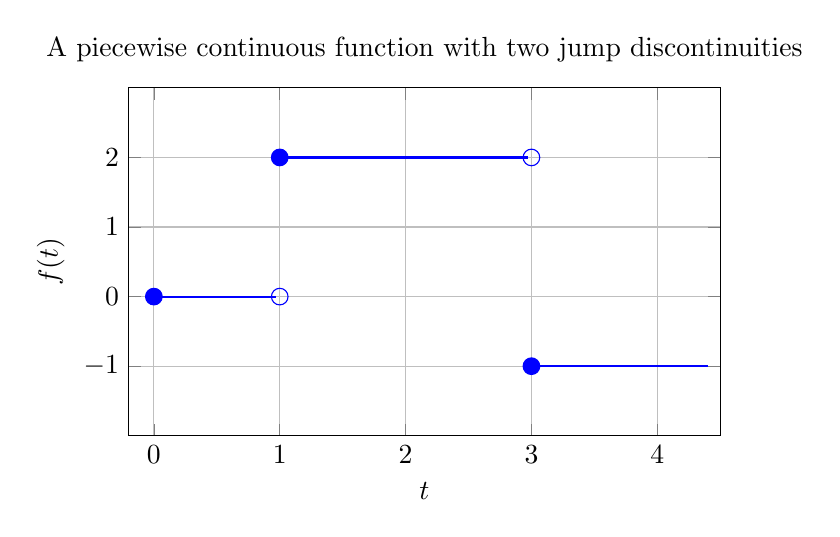
\begin{tikzpicture}
\begin{axis}[
  xlabel={$t$},
  ylabel={$f(t)$},
  xmin=-0.2, xmax=4.5,
  ymin=-2, ymax=3,
  grid=major,
  width=0.75\textwidth,
  height=6cm,
  title={A piecewise continuous function with two jump discontinuities},
  xtick={0,1,2,3,4},
  ytick={-1,0,1,2},
]
% Segment 1: f(t)=0 for 0 <= t < 1
\addplot[blue, thick, domain=0:0.97, samples=2] {0};
% Segment 2: f(t)=2 for 1 <= t < 3
\addplot[blue, thick, domain=1:2.97, samples=2] {2};
% Segment 3: f(t)=-1 for t >= 3
\addplot[blue, thick, domain=3:4.4, samples=2] {-1};

% Open circles at excluded endpoints
\addplot[blue, only marks, mark=o, mark size=3pt] coordinates {(1,0) (3,2)};
% Filled circles at included endpoints
\addplot[blue, only marks, mark=*, mark size=3pt] coordinates {(0,0) (1,2) (3,-1)};
\end{axis}
\end{tikzpicture}
\end{center}

\noindent At $t=1$ the function jumps from $0$ to $2$; at $t=3$ it jumps from $2$ to $-1$.
Both limits at each jump are finite, so this function is piecewise continuous on $[0, \infty)$.
Filled circles mark the value \emph{actually taken}; open circles mark the value
\emph{not taken}.

% =============================================================
\section{Functions of Exponential Order}
% =============================================================

\begin{infobox}{Definition: Exponential Order}
A function $f(t)$ is said to be of \textbf{exponential order} $\alpha$ if there exist constants
$M > 0$, $\alpha \in \mathbb{R}$, and $T \geq 0$ such that:
\[
  |f(t)| \leq M e^{\alpha t} \quad \text{for all } t \geq T.
\]
Intuitively: for large $t$, $f(t)$ must not grow faster than some exponential curve.
The smallest such $\alpha$ is called the \textbf{abscissa of convergence}.
\end{infobox}

\medskip
\noindent\textbf{Functions that ARE of exponential order:}

\begin{itemize}
  \item \textbf{Polynomials} $t^n$: for any $\epsilon > 0$,
        $t^n / e^{\epsilon t} \to 0$ as $t \to \infty$
        (exponential always beats polynomial), so $|t^n| \leq M e^{\epsilon t}$
        for large $t$. Exponential order $\alpha = \epsilon$ (any $\epsilon > 0$).
  \item $\sin t$, $\cos t$: bounded by $1$ for all $t$, so $|{\sin t}| \leq 1 = 1 \cdot e^{0 \cdot t}$.
        Exponential order $\alpha = 0$, $M = 1$.
  \item $e^{3t}$: $|e^{3t}| = 1 \cdot e^{3t}$, so $M = 1$, $\alpha = 3$. Exponential order~$3$.
\end{itemize}

\medskip
\noindent\textbf{Functions that are NOT of exponential order:}

\begin{itemize}
  \item $e^{t^2}$: Fix any $\alpha \in \mathbb{R}$.
        \[
          \frac{e^{t^2}}{e^{\alpha t}} = e^{t^2 - \alpha t} = e^{t(t - \alpha)} \to \infty
          \quad \text{as } t \to \infty,
        \]
        because for $t > \alpha$ the exponent $t(t-\alpha)$ grows without bound.
        Therefore $e^{t^2}$ \emph{cannot} be bounded by $M e^{\alpha t}$ for any fixed $\alpha$,
        and it is \textbf{not} of exponential order.
\end{itemize}

% =============================================================
\section{The Existence Theorem (Sufficient Condition)}
% =============================================================

\begin{infobox}{Theorem: Sufficient Conditions for Existence}
If $f(t)$ satisfies \emph{both} of the following:
\begin{enumerate}
  \item $f(t)$ is \textbf{piecewise continuous} on $[0, \infty)$, and
  \item $f(t)$ is of \textbf{exponential order} $\alpha$,
\end{enumerate}
then $\mathcal{L}\{f(t)\} = F(s) = \int_0^\infty e^{-st} f(t)\, dt$ \textbf{exists} for all
$s > \alpha$.
\end{infobox}

\medskip
\noindent\textbf{Proof Sketch.}
Split the integral at the constant $T$ from the exponential-order definition:
\[
  \int_0^\infty e^{-st} f(t)\, dt
  = \underbrace{\int_0^T e^{-st} f(t)\, dt}_{\text{(I)}}
  + \underbrace{\int_T^\infty e^{-st} f(t)\, dt}_{\text{(II)}}.
\]

\noindent\emph{Piece (I):}
On the finite interval $[0, T]$, piecewise continuity guarantees $f(t)$ is bounded and has
finitely many discontinuities, so the integral is finite.

\noindent\emph{Piece (II):}
Using $|f(t)| \leq M e^{\alpha t}$ for $t \geq T$,
\[
  \left|\int_T^\infty e^{-st} f(t)\, dt\right|
  \leq \int_T^\infty e^{-st} \cdot M e^{\alpha t}\, dt
  = M \int_T^\infty e^{-(s-\alpha)t}\, dt
  = \frac{M e^{-(s-\alpha)T}}{s - \alpha},
\]
which is \emph{finite} provided $s > \alpha$.
By the comparison test, piece (II) converges.

\medskip
Since both pieces are finite, $F(s)$ exists for all $s > \alpha$. \hfill $\square$

\medskip
\begin{infobox}{Important: Sufficient, Not Necessary}
The theorem gives a \textbf{sufficient} condition, not a necessary one.
A function can violate these conditions and still have a Laplace transform.
Classical example: $f(t) = t^{-1/2}$ has an integrable singularity at $t = 0$ (not piecewise
continuous there in the strict sense), yet
\[
  \mathcal{L}\{t^{-1/2}\} = \sqrt{\frac{\pi}{s}},
\]
which exists for $s > 0$ via the Gamma function connection.
\end{infobox}

% =============================================================
\section{Behaviour of $F(s)$ as $s \to \infty$}
% =============================================================

\begin{infobox}{Corollary: $F(s) \to 0$ as $s \to \infty$}
If $\mathcal{L}\{f(t)\} = F(s)$ exists for $s > \alpha$, then
\[
  \lim_{s \to \infty} F(s) = 0.
\]
\textbf{Justification:} As $s \to \infty$ the damping factor $e^{-st}$ crushes the integrand to
zero for every fixed $t > 0$, so the area under the integrand vanishes.

\medskip
\textbf{Sanity check:} If a computed $F(s)$ does NOT approach zero as $s \to \infty$, an error
was made somewhere in the computation.
\end{infobox}

\medskip
\begin{center}
\begin{tabular}{@{}llll@{}}
\toprule
\textbf{$f(t)$} & \textbf{$F(s)$} &
\textbf{$\lim_{s\to\infty} F(s)$} & \textbf{Passes check?} \\
\midrule
$1$              & $1/s$             & $0$ & Yes \checkmark \\
$e^{at}$         & $1/(s-a)$         & $0$ & Yes \checkmark \\
$\sin(\omega t)$ & $\omega/(s^2+\omega^2)$ & $0$ & Yes \checkmark \\
$t^n$            & $n!/s^{n+1}$      & $0$ & Yes \checkmark \\
(Erroneous) $F(s) = s/(s+1)$ & --- & $1 \neq 0$ & No $\times$ \\
\bottomrule
\end{tabular}
\end{center}

% =============================================================
\section{Worked Examples}
% =============================================================

\subsection*{Example 1: $f(t) = t^3$ is of exponential order}

\begin{infobox}{Example 1 --- $f(t) = t^3$}
\textbf{Claim:} $f(t) = t^3$ is of exponential order $\alpha$ for any $\alpha > 0$, and hence
$\mathcal{L}\{t^3\}$ exists.

\medskip
\textbf{Step 1.} We need to find $M > 0$, $\alpha > 0$, $T \geq 0$ such that
$t^3 \leq M e^{\alpha t}$ for $t \geq T$.

\medskip
\textbf{Step 2.} Take $\alpha = 1$.
Consider the ratio:
\[
  \frac{t^3}{e^t}.
\]
By L'H\^opital's rule applied three times (or by the standard limit theorem
``exponential beats polynomial''):
\[
  \lim_{t \to \infty} \frac{t^3}{e^t} = 0.
\]

\textbf{Step 3.} Since the limit is $0$, for any $\epsilon > 0$ (take $\epsilon = 1$)
there exists $T$ such that for all $t \geq T$:
\[
  \frac{t^3}{e^t} < 1 \implies t^3 < e^t = 1 \cdot e^{1 \cdot t}.
\]
So $M = 1$, $\alpha = 1$, $T$ as found above works.

\medskip
\textbf{Step 4.} Both conditions are satisfied: $t^3$ is continuous everywhere (certainly piecewise
continuous), and exponential order $1$ is established.
Therefore $\mathcal{L}\{t^3\}$ exists for all $s > 1$.
(The exact value is $\mathcal{L}\{t^3\} = 6/s^4$.)
\end{infobox}

\begin{learnbox}{What Did We Learn? (Example 1)}
Any polynomial $t^n$ is of exponential order for any $\alpha > 0$ because exponentials
always dominate polynomials as $t \to \infty$.
You can always take $M = 1$, $\alpha = \epsilon$ for any small $\epsilon > 0$.
\end{learnbox}

\subsection*{Example 2: $f(t) = e^{t^2}$ is NOT of exponential order}

\begin{infobox}{Example 2 --- $f(t) = e^{t^2}$}
\textbf{Claim:} $e^{t^2}$ is \emph{not} of exponential order, and therefore
$\mathcal{L}\{e^{t^2}\}$ does not exist.

\medskip
\textbf{Step 1.} Suppose for contradiction that $e^{t^2}$ is of exponential order $\alpha$, i.e.,
there exist $M > 0$ and $T \geq 0$ with $e^{t^2} \leq M e^{\alpha t}$ for all $t \geq T$.

\medskip
\textbf{Step 2.} Divide both sides by $e^{\alpha t}$ (positive):
\[
  e^{t^2 - \alpha t} \leq M \quad \text{for all } t \geq T.
\]

\medskip
\textbf{Step 3.} Examine the exponent $t^2 - \alpha t = t(t - \alpha)$.
For $t > \alpha$, the factor $(t - \alpha)$ is positive and grows without bound, so
$t(t - \alpha) \to +\infty$ as $t \to \infty$.
Hence $e^{t^2 - \alpha t} \to +\infty$, which \emph{cannot} be bounded by any constant $M$.

\medskip
\textbf{Step 4.} Contradiction. No such $M$ and $\alpha$ exist.
Therefore $e^{t^2}$ is \textbf{not} of exponential order, and
$\mathcal{L}\{e^{t^2}\}$ \textbf{does not exist}.
\end{infobox}

\begin{learnbox}{What Did We Learn? (Example 2)}
$e^{t^2}$ is the classic counterexample: its exponent is itself a function of $t$,
making it grow super-exponentially.
No brake $e^{-st}$ with a fixed $s$ can ever outrun it.
\end{learnbox}

\subsection*{Example 3: $f(t) = t^{-1/2}$ --- Singular but Transformable}

\begin{infobox}{Example 3 --- $f(t) = t^{-1/2}$}
\textbf{Issue:} $f(t) = t^{-1/2}$ has a singularity at $t = 0$ since
$\lim_{t \to 0^+} t^{-1/2} = +\infty$.
Strictly speaking, $f$ is \emph{not} piecewise continuous on $[0, T]$ for any $T > 0$
because the one-sided limit at $0$ is infinite --- the sufficient condition does not apply.

\medskip
\textbf{Does the transform exist anyway?}
Yes. Compute:
\[
  \mathcal{L}\{t^{-1/2}\} = \int_0^\infty e^{-st} t^{-1/2}\, dt.
\]
Substitute $u = st$ (so $t = u/s$, $dt = du/s$, $t^{-1/2} = (u/s)^{-1/2} = s^{1/2} u^{-1/2}$):
\[
  = \int_0^\infty e^{-u} \cdot s^{1/2} u^{-1/2} \cdot \frac{du}{s}
  = s^{-1/2} \int_0^\infty e^{-u} u^{-1/2}\, du
  = s^{-1/2} \cdot \Gamma\!\left(\tfrac{1}{2}\right)
  = \sqrt{\frac{\pi}{s}},
\]
using $\Gamma(1/2) = \sqrt{\pi}$ (a standard Gamma function result, stated without re-derivation).

\medskip
\textbf{Conclusion:} $\mathcal{L}\{t^{-1/2}\} = \sqrt{\pi/s}$ exists for $s > 0$.
The singularity at $0$ is \emph{integrable} (the area is finite despite the infinite spike),
so the transform still converges even though the sufficient condition is not satisfied.
\end{infobox}

\begin{learnbox}{What Did We Learn? (Example 3)}
The existence theorem gives a \emph{sufficient} condition.
Failing the piecewise continuity test at a single point does not automatically kill the
transform --- the singularity must be integrable.
Always check directly when the sufficient condition does not apply.
\end{learnbox}

% =============================================================
\section{Excel Example}
% =============================================================

This spreadsheet numerically demonstrates the contrast between a convergent integrand
($e^{-5t} \cdot t^3$) and a divergent one ($e^{-5t} \cdot e^{t^2}$), confirming what the
existence theorem predicts.

\medskip
\noindent\textbf{Spreadsheet layout} (columns A through C, rows 1 onward):

\medskip
\begin{center}
\begin{tabular}{@{}llll@{}}
\toprule
\textbf{Row} & \textbf{A: $t$} &
\textbf{B: $e^{-5t} \cdot t^3$} &
\textbf{C: $e^{-5t} \cdot e^{t^2}$} \\
\midrule
1 (header) & \texttt{t} & \texttt{exp(-5t)*t\^{}3} & \texttt{exp(-5t)*exp(t\^{}2)} \\
2 & 0.00 & \texttt{=EXP(-5*A2)*A2\^{}3} & \texttt{=EXP(-5*A2)*EXP(A2\^{}2)} \\
3 & 0.25 & \texttt{=EXP(-5*A3)*A3\^{}3} & \texttt{=EXP(-5*A3)*EXP(A3\^{}2)} \\
4 & 0.50 & \texttt{=EXP(-5*A4)*A4\^{}3} & \texttt{=EXP(-5*A4)*EXP(A4\^{}2)} \\
5 & 0.75 & \texttt{=EXP(-5*A5)*A5\^{}3} & \texttt{=EXP(-5*A5)*EXP(A5\^{}2)} \\
6 & 1.00 & \texttt{=EXP(-5*A6)*A6\^{}3} & \texttt{=EXP(-5*A6)*EXP(A6\^{}2)} \\
\bottomrule
\end{tabular}
\end{center}

\medskip
\noindent\textbf{Cell A2} $= 0$, \textbf{A3} $= 0.25$, \ldots
Fill A2:A14 with $t = 0, 0.25, 0.5, \ldots, 3.0$ in steps of $0.25$.

\medskip
\noindent\textbf{Sample computed values} (approximate):

\medskip
\begin{center}
\begin{tabular}{@{}rll@{}}
\toprule
$t$ & $e^{-5t} \cdot t^3$ & $e^{-5t} \cdot e^{t^2}$ \\
\midrule
0.00  & 0.000000       & 1.000000   \\
0.50  & 0.000474       & 1.284025   \\
1.00  & 0.006738       & 40.343     \\
1.50  & 0.003355       & 35957      \\
2.00  & 0.000490       & \texttt{\#NUM!} (overflow) \\
3.00  & 0.000000       & \texttt{\#NUM!} (overflow) \\
\bottomrule
\end{tabular}
\end{center}

\medskip
Column B shrinks steadily toward zero --- the exponential damping wins.
Column C explodes to overflow (the exponential order condition is violated by $e^{t^2}$).

\medskip
\noindent\textbf{Verify the exact value:}
$\mathcal{L}\{t^3\}\big|_{s=5} = 6/5^4 = 6/625 = 0.0096$.
Numerically integrate column B (using the Trapezoidal Rule or \texttt{=SUMPRODUCT}) over
$t = 0$ to $t = 3$ with step $0.25$ and confirm the result is close to $0.0096$.

\begin{learnbox}{What Did We Learn? (Excel)}
Column B (convergent integrand) shrinks to zero as $t$ grows, confirming the Laplace integral
will be finite.
Column C (divergent integrand) explodes at moderate values of $t$, confirming that
$\mathcal{L}\{e^{t^2}\}$ cannot exist.
The spreadsheet provides direct numerical evidence for what the existence theorem says
analytically.
\end{learnbox}

% =============================================================
\section{Python Example}
% =============================================================

\begin{lstlisting}[language=Python, caption={Numerical check of convergence vs.\ divergence}]
import numpy as np
from scipy import integrate

s = 5  # chosen value of s

# --- Convergent integrand: exp(-5t) * t^3 ---
def integrand_convergent(t):
    return np.exp(-s * t) * t**3

# Exact value: 6 / s^4
exact = 6 / s**4
print(f"Exact value: 6/s^4 = 6/{s**4} = {exact:.8f}")

for T in [5, 10, 20]:
    val, err = integrate.quad(integrand_convergent, 0, T)
    print(f"  Numerical integral (0 to {T:2d}): {val:.8f}  [error est. {err:.2e}]")

# Expected output:
# Exact value: 6/s^4 = 6/625 = 0.00960000
#   Numerical integral (0 to  5): 0.00959978  [error est. 4.51e-12]
#   Numerical integral (0 to 10): 0.00960000  [error est. 5.33e-13]
#   Numerical integral (0 to 20): 0.00960000  [error est. 5.33e-13]

print()

# --- Divergent integrand: exp(-5t) * exp(t^2) ---
def integrand_divergent(t):
    return np.exp(-s * t) * np.exp(t**2)

print("Attempting to integrate exp(-5t)*exp(t^2) from 0 to T:")
for T in [2, 3, 5]:
    try:
        val, err = integrate.quad(integrand_divergent, 0, T,
                                   limit=100, epsabs=1e-4, epsrel=1e-4)
        print(f"  T={T}: value = {val:.4e}  (note: very large, growing)")
    except Exception as e:
        print(f"  T={T}: Integration failed -- {e}")

# Expected output:
# Attempting to integrate exp(-5t)*exp(t^2) from 0 to T:
#   T=2: value = 3.5941e+04  (note: very large, growing)
#   T=3: value = 2.7407e+12  (note: very large, growing)
#   T=5: Integration failed -- or returns overflow/IntegrationWarning
\end{lstlisting}

\begin{learnbox}{What Did We Learn? (Python)}
The numerical integration of $e^{-5t} \cdot t^3$ converges quickly and matches the exact
value $6/625 = 0.0096$ to many decimal places, even by $T = 10$.
In contrast, $e^{-5t} \cdot e^{t^2}$ produces enormous values even for moderate $T$,
confirming divergence and the absence of a Laplace transform.
\end{learnbox}

% =============================================================
\section{Viva-Style Oral Questions}
% =============================================================

\begin{enumerate}[label=\textbf{Q\arabic*.}]

\item \textbf{Define piecewise continuous function.} \\
\textbf{Answer:} A function $f(t)$ is piecewise continuous on $[0, \infty)$ if on every finite
interval $[0, T]$ it has at most finitely many jump discontinuities and both one-sided limits
exist and are finite at each discontinuity.

\item \textbf{Define exponential order $\alpha$.} \\
\textbf{Answer:} $f(t)$ is of exponential order $\alpha$ if there exist $M > 0$, $T \geq 0$ such
that $|f(t)| \leq M e^{\alpha t}$ for all $t \geq T$. The function must not grow faster than
some exponential for large $t$.

\item \textbf{State the sufficient conditions for existence of $\mathcal{L}\{f(t)\}$.} \\
\textbf{Answer:} If (i) $f(t)$ is piecewise continuous on $[0, \infty)$ and (ii) $f(t)$ is of
exponential order $\alpha$, then $\mathcal{L}\{f(t)\}$ exists for all $s > \alpha$.

\item \textbf{Why is the existence theorem called a sufficient condition and not a necessary one?} \\
\textbf{Answer:} A function can fail one or both conditions yet still have a Laplace transform.
For example, $t^{-1/2}$ violates piecewise continuity at $t = 0$ (the limit is $+\infty$), yet
$\mathcal{L}\{t^{-1/2}\} = \sqrt{\pi/s}$ exists. The theorem guarantees existence when the
conditions hold but does not rule it out otherwise.

\item \textbf{What does $F(s) \to 0$ as $s \to \infty$ tell us?} \\
\textbf{Answer:} It is a necessary consequence of the Laplace transform: for large $s$ the
damping $e^{-st}$ kills the integrand. If a computed $F(s)$ does not go to zero as $s \to \infty$,
the computation contains an error.

\item \textbf{Why does $e^{t^2}$ have no Laplace transform?} \\
\textbf{Answer:} Because $e^{t^2}$ is not of exponential order. For any fixed $\alpha$,
$e^{t^2}/e^{\alpha t} = e^{t^2 - \alpha t} \to \infty$ as $t \to \infty$, so no bound
$M e^{\alpha t}$ can contain $e^{t^2}$. Without the exponential order condition, the integral
$\int_0^\infty e^{-st} e^{t^2}\, dt$ diverges for every $s$.

\item \textbf{What is the role of the constants $M$ and $\alpha$ in the definition of exponential order?} \\
\textbf{Answer:} $\alpha$ sets the rate of the bounding exponential, specifying how fast $f(t)$
is allowed to grow. $M > 0$ is a scaling constant that handles any finite initial transient
(the bound is only required for $t \geq T$). Together they assert $f(t)$ eventually lies below
the curve $M e^{\alpha t}$.

\item \textbf{Why does $f(t) = 1/t$ fail the piecewise continuity condition?} \\
\textbf{Answer:} At $t = 0$, $\lim_{t \to 0^+} (1/t) = +\infty$. The one-sided limit is
\emph{infinite}, not finite. Piecewise continuity requires both one-sided limits to be finite at
every discontinuity, so $1/t$ fails this condition on any interval $[0, T]$ that includes~$0$.

\end{enumerate}

% =============================================================
\section{Descriptive Questions}
% =============================================================

\begin{enumerate}[label=\textbf{D\arabic*.}]

\item \textbf{State and prove (sketch) the sufficient conditions for the existence of
$\mathcal{L}\{f(t)\}$.} \\
\textit{Expected answer:} State both conditions, split the integral at $T$, bound piece (II)
using $|f(t)| \leq M e^{\alpha t}$, apply the comparison test to obtain convergence for $s > \alpha$.

\item \textbf{Show that $f(t) = e^{3t} \sin(2t)$ is of exponential order and hence has a Laplace
transform. Find suitable values of $M$ and $\alpha$.} \\
\textit{Expected answer:} $|e^{3t} \sin(2t)| \leq e^{3t} \cdot 1 = 1 \cdot e^{3t}$.
So $M = 1$, $\alpha = 3$. Since the function is also continuous (hence piecewise continuous),
the existence theorem guarantees $\mathcal{L}\{e^{3t}\sin(2t)\}$ exists for $s > 3$.

\item \textbf{Explain, using the comparison test, why $\int_T^\infty e^{-(s-\alpha)t}\, dt$
converges for $s > \alpha$, and how this forms the key step in the proof of the existence
theorem.} \\
\textit{Expected answer:} For $s > \alpha$, $(s-\alpha) > 0$, so
$\int_T^\infty e^{-(s-\alpha)t}\, dt = e^{-(s-\alpha)T}/(s-\alpha) < \infty$.
Since the integrand $|e^{-st} f(t)| \leq M e^{-(s-\alpha)t}$ and the bounding integral
converges, by the comparison test the original integral also converges.

\item \textbf{Explain the distinction between necessary and sufficient conditions with a concrete
example in the context of Laplace transforms.} \\
\textit{Expected answer:} A sufficient condition means: if $P$ holds then $Q$ holds, but $Q$
may hold without $P$. The existence theorem is sufficient: piecewise continuity plus exponential
order $\Rightarrow$ transform exists. But $t^{-1/2}$ (not piecewise continuous at 0) still has
transform $\sqrt{\pi/s}$, proving the conditions are not necessary.

\item \textbf{Explain the sanity check $\lim_{s \to \infty} F(s) = 0$ with two examples --- one
function that passes and one (erroneous) expression that fails.} \\
\textit{Expected answer:} For $\mathcal{L}\{e^{2t}\} = 1/(s-2)$:
$\lim_{s\to\infty} 1/(s-2) = 0$. Passes.
If someone mistakenly obtains $F(s) = s/(s+3)$:
$\lim_{s\to\infty} s/(s+3) = 1 \neq 0$. Fails --- indicating an error in the derivation.

\end{enumerate}

% =============================================================
\section{Practice Problems}
% =============================================================

For each of the following functions, determine: (a) whether it is of exponential order,
(b) whether $\mathcal{L}\{f(t)\}$ is guaranteed to exist by the sufficient condition,
and (c) the abscissa of convergence $\alpha$ if applicable.

\begin{enumerate}[label=\textbf{P\arabic*.}]

\item $f(t) = t^5$ \\
\textit{Hint:} Polynomial; exponential beats $t^5$ for any $\alpha > 0$. $\mathcal{L}\{t^5\}$
exists for $s > 0$; exact value $= 120/s^6$.

\item $f(t) = e^{3t} \sin t$ \\
\textit{Hint:} $|e^{3t}\sin t| \leq e^{3t}$; exponential order $3$.
$\mathcal{L}\{e^{3t}\sin t\} = 1/[(s-3)^2+1]$ for $s > 3$.

\item $f(t) = \cosh(t^2)$ \\
\textit{Hint:} $\cosh(t^2) = (e^{t^2} + e^{-t^2})/2 \geq e^{t^2}/2$.
Since $e^{t^2}$ is not of exponential order, neither is $\cosh(t^2)$.
$\mathcal{L}\{\cosh(t^2)\}$ does not exist.

\item $f(t) = \ln(1 + t)$ \\
\textit{Hint:} $\ln(1+t) < t$ for $t > 0$, and $t \leq e^{\epsilon t}$ for any $\epsilon > 0$.
So $\ln(1+t)$ is of exponential order $\epsilon$ (any $\epsilon > 0$); transform exists
for $s > 0$.

\item $f(t) = t^{-1/2}$ \\
\textit{Hint:} Singular at $t = 0$; sufficient condition technically fails.
However, the singularity is integrable and $\mathcal{L}\{t^{-1/2}\} = \sqrt{\pi/s}$ exists for
$s > 0$ via direct calculation.

\item $f(t) = e^{-t^2}$ \\
\textit{Hint:} $e^{-t^2} < 1 = 1 \cdot e^{0 \cdot t}$; exponential order $0$ with $M=1$.
$\mathcal{L}\{e^{-t^2}\}$ exists for $s > 0$ (its exact form involves the error function).

\end{enumerate}

% =============================================================
\section{Multiple Choice Questions}
% =============================================================

\begin{enumerate}[label=\textbf{MCQ \arabic*.}]

\item Which of the following is the correct definition of exponential order $\alpha$?
\begin{enumerate}[label=(\alph*)]
  \item $f(t) \to 0$ as $t \to \infty$
  \item \textbf{There exist $M > 0$ and $T \geq 0$ such that $|f(t)| \leq M e^{\alpha t}$ for all $t \geq T$}
  \item $f(t)$ is bounded on $[0, \infty)$
  \item $f(t) = e^{\alpha t}$ for large $t$
\end{enumerate}
\textit{Explanation:} Option (b) is the standard definition. (a) and (c) are more restrictive
(they only work for $\alpha < 0$ or $\alpha = 0$); (d) confuses equality with an upper bound.

\item The existence theorem for $\mathcal{L}\{f(t)\}$ requires which two conditions?
\begin{enumerate}[label=(\alph*)]
  \item Differentiability and bounded derivative
  \item Continuity and periodicity
  \item \textbf{Piecewise continuity and exponential order}
  \item Integrability on every $[0, T]$ and monotone decrease
\end{enumerate}
\textit{Explanation:} The theorem (as stated in most engineering mathematics texts) requires
piecewise continuity on $[0,\infty)$ and exponential order $\alpha$.

\item If $\mathcal{L}\{f(t)\} = F(s)$ exists, what is $\lim_{s \to \infty} F(s)$?
\begin{enumerate}[label=(\alph*)]
  \item $+\infty$
  \item $f(0)$
  \item $1$
  \item \textbf{$0$}
\end{enumerate}
\textit{Explanation:} As $s \to \infty$, the factor $e^{-st}$ suppresses the integrand to zero
for every $t > 0$, forcing $F(s) \to 0$. This is a necessary consequence of the existence of
the transform.

\item Which function does NOT have a Laplace transform?
\begin{enumerate}[label=(\alph*)]
  \item $t^{100}$
  \item $e^{1000t}$
  \item $t^{-1/2}$
  \item \textbf{$e^{t^2}$}
\end{enumerate}
\textit{Explanation:} $t^{100}$, $e^{1000t}$, and $t^{-1/2}$ all have Laplace transforms.
$e^{t^2}$ is not of exponential order (its growth outpaces every fixed exponential), so its
transform does not exist.

\item A function $f(t)$ has infinitely many jump discontinuities on $[0, 1]$, all with finite
one-sided limits. Which statement is TRUE?
\begin{enumerate}[label=(\alph*)]
  \item $f(t)$ is piecewise continuous on $[0,1]$
  \item $f(t)$ is piecewise continuous only if the jumps decrease to 0
  \item \textbf{$f(t)$ is NOT piecewise continuous on $[0,1]$ (infinitely many jumps are not allowed)}
  \item $f(t)$ is piecewise continuous because all limits are finite
\end{enumerate}
\textit{Explanation:} Piecewise continuity requires \emph{finitely many} jump discontinuities
on any bounded interval. Infinitely many jumps on $[0,1]$ violate this, even if each individual
limit is finite.

\end{enumerate}

% =============================================================
\section{Common Mistakes}
% =============================================================

\begin{mistakebox}{Common Mistakes in Conditions for Existence}
\begin{tabular}{@{}p{0.28\textwidth} p{0.30\textwidth} p{0.30\textwidth}@{}}
\toprule
\textbf{Mistake} & \textbf{What Students Do} & \textbf{Correct Approach} \\
\midrule
Treating the existence theorem as necessary &
Concluding a function has no Laplace transform purely because it fails the piecewise continuity
or exponential order test &
Check directly: the conditions are sufficient only.
Functions like $t^{-1/2}$ fail the sufficient test yet do have transforms. \\
\midrule
Confusing ``exponential order'' with ``grows exponentially everywhere'' &
Claiming $e^{3t}$ is NOT of exponential order because it grows, or claiming every
increasing function fails &
Exponential order means bounded above by $Me^{\alpha t}$ for large $t$.
$e^{3t}$ trivially satisfies $|e^{3t}| \leq 1 \cdot e^{3t}$. \\
\midrule
Ignoring discontinuities when checking piecewise continuity &
Checking only that a function is ``mostly continuous'' without listing and classifying its
discontinuities &
On every $[0,T]$, count all discontinuities; verify both one-sided limits are finite at each. \\
\midrule
Not checking behaviour at $t = 0$ for singular functions &
Writing ``$1/t$ is piecewise continuous on $[0,\infty)$'' &
$1/t$ has an infinite discontinuity at $t = 0$.
Always check the endpoints of the interval including $t = 0$. \\
\midrule
Assuming all bounded functions automatically have transforms &
Arguing that since $\sin(1/t)$ is bounded ($|\sin(\cdot)| \leq 1$), its transform exists &
Bounded is not the same as piecewise continuous.
$\sin(1/t)$ oscillates infinitely near $t = 0$; the limit does not exist there. \\
\bottomrule
\end{tabular}
\end{mistakebox}

% =============================================================
\section{Quick Recap}
% =============================================================

\begin{learnbox}{Quick Recap: Conditions for Existence of $\mathcal{L}\{f(t)\}$}
\begin{itemize}
  \item \textbf{Piecewise continuity:} On every $[0,T]$, $f(t)$ has finitely many jumps and both
        one-sided limits are finite at each jump.
  \item \textbf{Exponential order $\alpha$:} $|f(t)| \leq M e^{\alpha t}$ for all large $t$;
        the function must not outgrow every exponential.
  \item \textbf{Existence theorem (sufficient):} If $f(t)$ is piecewise continuous AND of
        exponential order $\alpha$, then $\mathcal{L}\{f(t)\}$ exists for all $s > \alpha$.
  \item \textbf{Sufficient, not necessary:} Failing the conditions does not prove
        non-existence --- $t^{-1/2}$ is the canonical counterexample.
  \item \textbf{Sanity check:} Any valid $F(s) = \mathcal{L}\{f(t)\}$ must satisfy
        $\lim_{s \to \infty} F(s) = 0$.
  \item \textbf{Classic counterexample:} $e^{t^2}$ is \emph{not} of exponential order because
        $e^{t^2}/e^{\alpha t} = e^{t(t-\alpha)} \to \infty$ for any fixed $\alpha$.
  \item \textbf{Brake analogy:} $e^{-st}$ is a brake on $f(t)$.
        Exponential order ensures the brake wins for large $t$; $e^{t^2}$ accelerates faster
        than any brake can stop.
  \item \textbf{Region of convergence:} $F(s)$ is defined and analytic for $s > \alpha$, where
        $\alpha$ is the abscissa of convergence determined by the exponential order of $f$.
\end{itemize}
\end{learnbox}

\end{document}
